% !TeX engine = xelatex
\documentclass{ctexbeamer}
\usepackage{ctex}
\usepackage{booktabs}
\usepackage{svg}
\usepackage{pdfpages}
\usepackage{fontspec}
\usepackage{fontawesome}
\usepackage[style=authortitle-comp,backend=bibtex]{biblatex}
\usecolortheme{seagull}
\setbeamertemplate{sidebar right}{}
\setbeamertemplate{footline}{%
	\hfill\usebeamertemplate***{navigation symbols}
	\hspace{1cm}\insertframenumber{}/\inserttotalframenumber}
\title{针对时间序列分类(TSC)的深度模型}
\subtitle{Deep Learning for Time Series Classification \footfullcite{fawaz2019deep}}
\author{Xinyi Li}
\date{\today}

\addbibresource{ref.bib}

\begin{document}
\begin{frame}
	\titlepage
\end{frame}

\begin{frame}{Overview}
  \tableofcontents
\end{frame}

\section{问题背景描述}
\begin{frame}{Different Learning Tasks}
	\begin{columns}

		\column{.47\textwidth}
		Univariate

		\column{.47\textwidth}
		Multi-variate
		\begin{block}{MTS}
			\begin{itemize}
				\item different measurements of the \textbf{same} instance
				\item \textbf{high correlation}
				\item feeding features
			\end{itemize}
		\end{block}

		\begin{block}{panel data}
			\begin{itemize}
				\item the same measurements on \textbf{different} instances
				\item i.i.d. assumption
				\item feeding sku/store/...
			\end{itemize}
		\end{block}
	\end{columns}
\end{frame}

\begin{frame}{Problem Description}
	\framesubtitle{univariance/multi-variance/panel}
	\begin{center}
		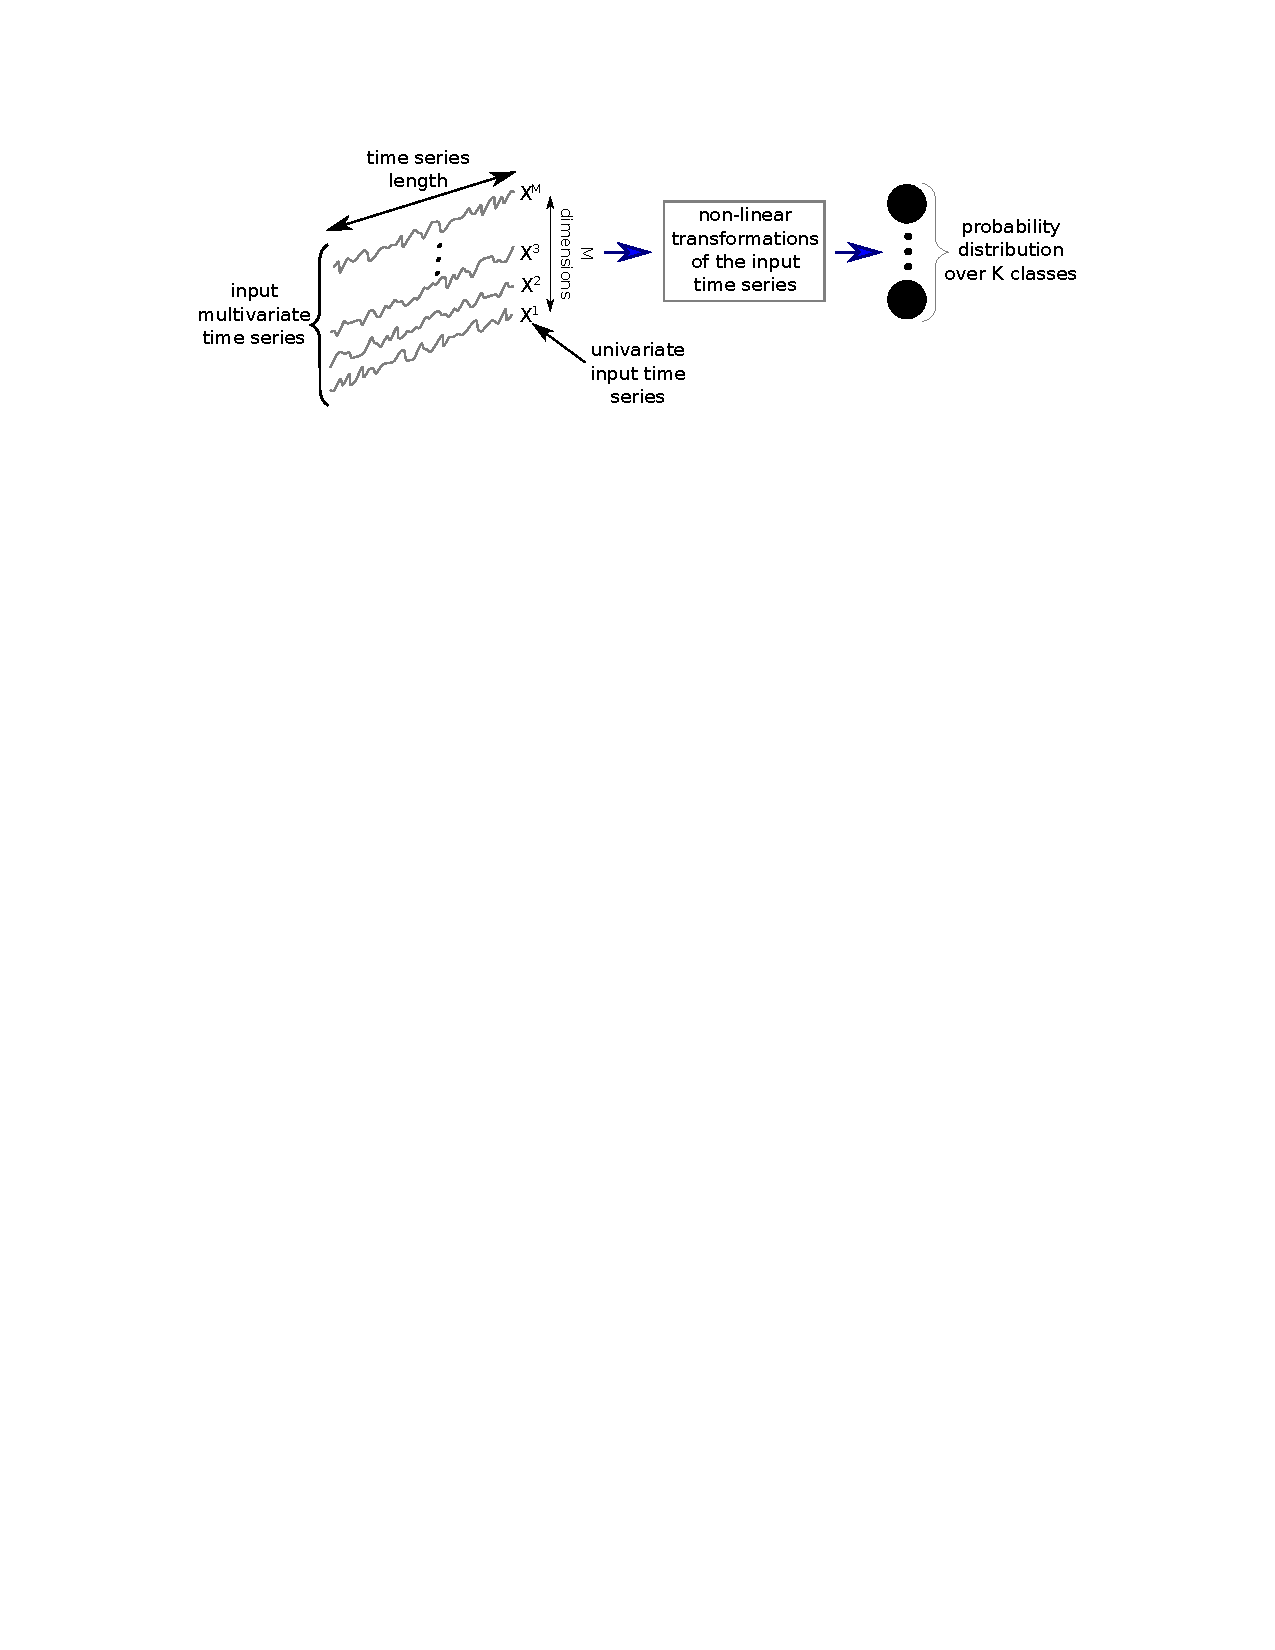
\includegraphics[width=\textwidth]{figure/base_formula}
	\end{center}
\end{frame}

\section{Strong Baseline}
\begin{frame}{HIVE-COTE\footfullcite{lines2016hive}:}
	\framesubtitle{\textbf{SOTA} classic algorithm \footfullcite{bagnall2017great}: Collective of Transformation based \textbf{Ensembles} (COTE) with a Hierarchical Vote system}
	\begin{enumerate}
		\item Elastic Ensemble(\textbf{EE}): combination of 1-NN classifiers using different measurements
		\item Shapelet Transform Ensemble(\textbf{ST}): top $k$ shaplets (independent phase short pattern)
		\item Bag-of-SFA-Symbols (\textbf{BOSS}) Ensemble: shapelets based on presence or absence
		\item Time Series Forest (\textbf{TSF}): trained on selected $3 \sqrt{m}$ features
		\item Random Interval Features (\textbf{RIF}): spectral component of \textit{Flat-COTE}
	\end{enumerate}
\end{frame}

\begin{frame}{HIVE-COTE Algorithm\footnote{\url{https://github.com/TonyBagnall/py-hive-cote}}}
	\framesubtitle{ensemble of ensembles}
	Refs to Flat-COTE
	\begin{center}
		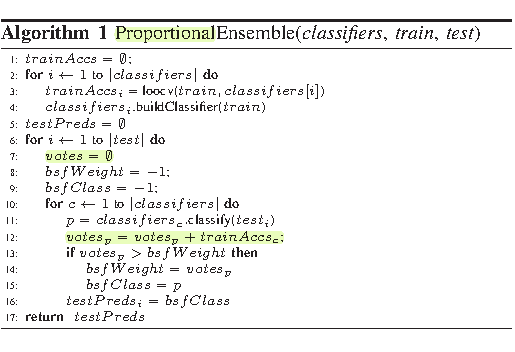
\includegraphics[width=.95\textwidth]{figure/flat_cote_algo}
	\end{center}

\end{frame}

\section{TSC社区生态}

\begin{frame}{Libraries/Implements/Community}
  \framesubtitle{sktime\footfullcite{sktime} \& its extensions}
  \href{https://github.com/alan-turing-institute/sktime}{\Large{Sktime}}
  \begin{itemize}
    \item based on classic models (shallow)
    \item \texttt{scikit-learn} interface compatible
  \end{itemize}
  \href{https://github.com/sktime/sktime-dl}{\Large{Sktime-dl}}
  \begin{itemize}
    \item use \texttt{Keras} to implement all 9 \textbf{SOTA} deep models above
    \color{red}{\item 暂时\textbf{不能}直接安装(MacOS)}
  \end{itemize}
  \href{http://www.timeseriesclassification.com/}{\Large{UEA \& UCR Time Series Classification Repository}}
  \begin{itemize}
    \item 128 TSC datasets + 30 MTS datasets
    \item Collect a bunch of \textbf{classic} algorithms
  \end{itemize}
\end{frame}

\begin{frame}{MLP/DNN}
	\framesubtitle{Multi Layer Perceptrons/Fully-Connected(FC) Network}
	The Simplest DNN (e.g. \texttt{keras.Layers.Dense})
	$$\mathbf{X}_{i+1} = \sigma (\mathbf{W}_i \mathbf{X}_i + b_i)$$
	Final ($l$-th) layer activate function: softmax
	$$\hat {y} _{k} (\mathbf{X}_{l-1}) = (e^{\mathbf{W}_k \mathbf{X}_{l-1} + b_k}) /
	(\sum_{i=1}^{K} {e^{\mathbf{W}_i \mathbf{X}_{l-1} + b_i}})$$
	Objective loss:  categorical cross entropy
	$$Loss(\textbf{X}) = - \sum_{i=1}^{K}{y_i} \log {\hat y}_i$$
	minimized to learn the weights using \textbf{gradient descent} method
\end{frame}

\begin{frame}{FCNN\footfullcite{gamboa2017deep}}
	\framesubtitle{Fully Convolutional Neural Network}
	\begin{center}
		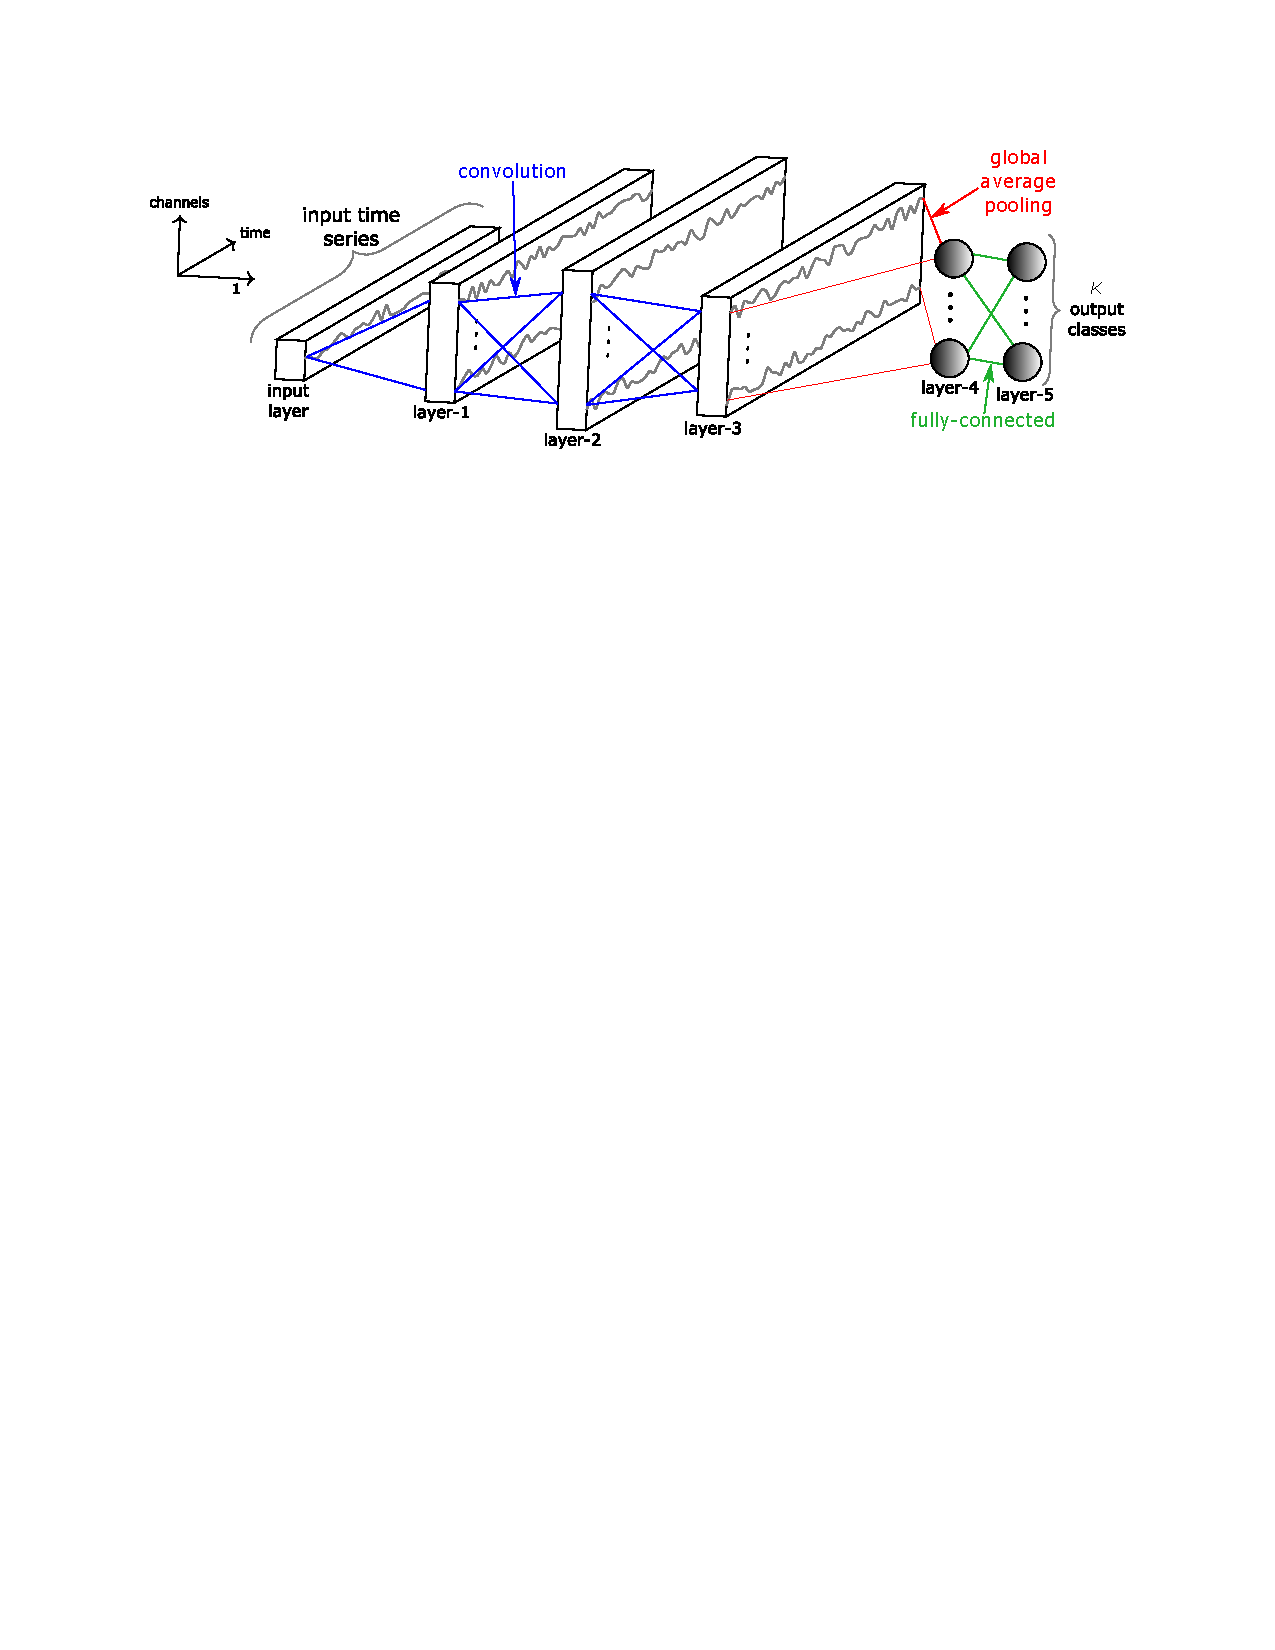
\includegraphics[width=1.05\textwidth]{figure/fcnn}
	\end{center}
	convolution layer ($\forall$ time stamp $t$ shares filter $\color{blue}{\omega}$ with length $l$)
	$$\mathbf{C}_t = \sigma ({\color{blue}{\omega}}* \mathbf{X}_{t-l/2:t+l/2} + {\color{blue}{b}}) | \forall t \in [1,T ]$$
\end{frame}


\begin{frame}{}
  \begin{center}
  {\Huge{Thanks}} \\
  All codes, slides and papers available\\
  \faGithub \href{https://github.com/li-xin-yi/deep_time_series_share_slide}{li-xin-yi/deep\_time\_series\_share\_slide}
\end{center}
\end{frame}

\end{document}
